\chapter{Analysis}

The analysis is a very important part of the whole project. It helps us to understand what is excepted from the system and how we will try to fulfil these expectations. There are many methodologies in area of software engineering but you have to do the analysis before you start to write the code no matter which methodology you choose. The analysis doesn't have to be big (especially in an agile methodology) but it has to be there.

In this chapter there is analysis of desired functionality, used frameworks and development environment. The most important part is the analysis of desired functionality because it helps to understand what is and what is not excepted from this project. The analysis of used frameworks is based on desired functionality because used framework has to be able to help with its realisation.

\section{Desired Functionality}

There are a lot of applications that provides the class modeling. Basic appearance is mostly common. There is a space where the model is shown (this space will be called workspace) and some toolbox where user can choose the tool he wants.

Every class diagram modeller has to be able to depict the basic elements of the class diagram as were described in section \ref{section:classDiagramDescription}. Existing modellers provides another functionality like information about complexities of single classes, their constraints, statuses, requirements, notes and many others. It is a lot of functionality that can not be created during a one bachelor project but it can be implemented in a related project.

Main aim of this project is to implement a metamodel of the class diagram. Developers of CASE system does not treat UML diagrams like diagrams. For them, the basics of UML diagram is the metamodel and the diagram is only its graphical representation. The metamodel represents the structure of the diagram and is standardly represented by an UML class diagram. The metamodel is not used only in conjunction with UML diagrams. The metamodel can be used to represent the abstraction of any other problem. The reason why I use the metamodel in conjunction with the UML diagram is that the OMG\footnote{OMG - Object Management Group - is a consortium which created (among others) the UML specification.} defined its UML standard by use of metamodel. The structure of the metamodel that will be implemented in this project is described in next section \ref{section-metamodel}.

A feature that is not a common one and is implemented in the Indepmod Class Notation Modeller is an annotation modelling. It provides the ability to assign annotations to classes, methods and attributes. Annotations are used in the Java programming language from version 1.5 and in the C\# programming language. Annotations are form of metadata which are stored in the source code. Alternative to annotations are configuration files (very often of XML type) that hold these information. These metadata are often used by frameworks. An example can be the JPA\footnote{JPA - Java Persistence API} framework of Java EE\footnote{Java EE - Java Enterprise Edition} that uses these metadata for the definition of object relation mapping (ORM)\footnote{Object Relation Mapping - a technique that maps objects from object oriented system into tables from relation database}. In a former version of java, these metadata were stored in XML configuration files. When there was a lot of classes to be configured, these configuration files were very large and confusing. On the other hand, annotations allow to specify these configurations inside the classes. This means that if you want to see or edit a class configuration, you don't have to search it in a file with maybe hundreds or thousands lines. Instead, you will open a desired class and find these information right there.

Annotations are nowadays very often used. The annotation modeling feature brings the advantage that a developer can create these annotations during a class modelling. When he creates the code (lets the case system to generate it) from the diagram he will have these annotation right there. If the case system were not able to model annotations, the developer would have to take a look at the diagram, remember which annotations should be where and add them into the code manually. Of course, this should be repeated when the model is changed.

The Indepmod Class Diagram Plugin will be also able to provide its diagram data to another Netbean's plugin. It means that there could be a plugin which will be able to e.g. generate a code according to the model or create an report. This will be done by some public API\footnote{API - Application Programming Interface} which will be provided by this application. This API will provide the type of the diagram (class or business diagram), the information about elements of the diagram and the picture of the diagram. The picture can be used by another plugin for example for a report. Concrete implementation of the API will be described in the Architecture chapter, concrete in the section \ref{section:classModelAPI}.

At the end of this section I would like to recapitulate three main requirements on the Indepmod Class Diagram Plugin. These requirements are:
\begin{itemize}
    \item Implement the standard class diagram modelling tool,
    \item it will also have a special feature for annotation modelling,
    \item created model will be provided to other Netbeans plugin by an public API.
\end{itemize}

\subsection{Class Diagram Metamodel}
\label{section-metamodel}

\begin{figure}[!ht]
\begin{center}
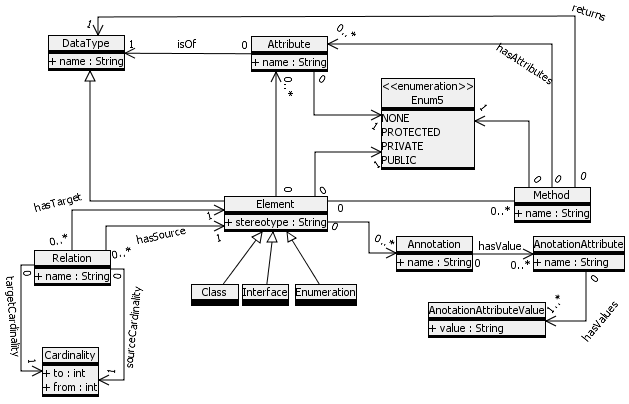
\includegraphics[scale=1]{img/classDiagramMetamodel.png}
\caption{Class Diagram Metamodel}
\label{f-classDiagramMetamodel}
\end{center}
\end{figure}

Figure \ref{f-classDiagramMetamodel} shows the metamodel of the class diagram that Indepmod Class Notation uses. From this metamodel you can see what the Indepmod Class Notation can and what it can not. Main building block of whole class diagram is an Element. The Element can be a Class, an Interface or an Enumeration. Every Element has a visibility, a stereotype (which can be empty) and a name. Each Element defines a data type identified by its name. In addition to the stereotype and the name, the Element has also the list of annotations, attributes and methods.

An Attribute has a name, a visibility and represents a data type. This data type can be the data type of an Element that we have already created or it can be another else data type (like String or int data type in Java). The Attribute can also have several (or none) Annotations. A Method is also defined by a name and has a visibility. The Attributes owned by the Method represents the parameters and the data type represents what the method returns. An Annotation has a name and can have several Annotation Attributes. Each Annotation Attribute has the name and a list of values.

\subsection{Model Type}

The Indepmod Class Notation Plugin will allow to create two types of class model. The first one is a standard Class model which has been already described in the section \ref{section:classDiagramDescription}. The second one is a business model. The selection of desired diagram in the application type will be done when user creates a new diagram. 

The purpose of the business model has been also described in the section \ref{section:classDiagramDescription}. Business model does not use all elements of the class model. It uses classes, its attributes and relations between classes. A class represents an entity from the problem domain. An attribute describes a property of the entity and a relation represents exactly what its name says - the relation between entities. An example of the business model can be the Figure \ref{f-classDiagramMetamodel}, which describes the problem domain of the class model.
